\section{Methodology}
\label{sec:method}

\subsection{System Overview}
The proposed framework operates in two distinct stages (Fig.~\ref{fig:pipeline}). In Stage~1, the denoiser \HSL{} is trained on 8192-sample segments in raw physical millivolt units ($\mathrm{mV}$) to reconstruct clean waveforms without distorting intrinsic signal distributions. In Stage~2, the weights of \HSL{} are frozen, and the model is utilized as an upstream signal purifier for downstream cardiac arrhythmia classification. Extracted 256-sample cardiac beats are normalized and fed into \RRN{}, which fuses morphological features with a 6-dimensional RR timing pathway.

\subsection{Data Preparation and Noise Model}
\label{sec:preproc}
Single-lead MIT-BIH recordings ($f_s = 360$\,Hz) are first passed through a zero-phase Butterworth bandpass filter ($0.67$--$100$\,Hz), which removes baseline drift and high-frequency interference without shifting the R-peaks in time. The filtered signals are divided into segments of $L = 8192$ samples ($22.75$\,s) with $50\%$ overlap, and segments whose energy lies outside the 5th--95th percentile range are discarded to remove flatlines and sensor detachment. The remaining segments serve as the clean references $x_0[n]$.

\paragraph*{Physiological Noise Model}
To faithfully emulate clinical environments, realistic noise waveforms from the MIT-BIH Noise Stress Test Database (NSTDB) are superimposed onto clean segments $x_0[n]$:
\begin{equation}
x[n] = x_0[n] + a \sum_{k \in K} \eta_k[n], \quad a = \sqrt{\frac{P_{x_0}}{10^{\mathrm{SNR}/10} P_{\eta}}},
\label{eq:noise_model}
\end{equation}
where $K \subseteq \{\mathrm{bw}, \mathrm{ma}, \mathrm{em}\}$ denotes a subset comprising single, double, or triple noise sources, $P$ represents mean squared power, and $\mathrm{SNR} \in \{-10, -7, -5, -3, 0, 1, 3, 5, 7, 10\}$\,dB controls the contamination severity.

\begin{figure}[!t]
\centering
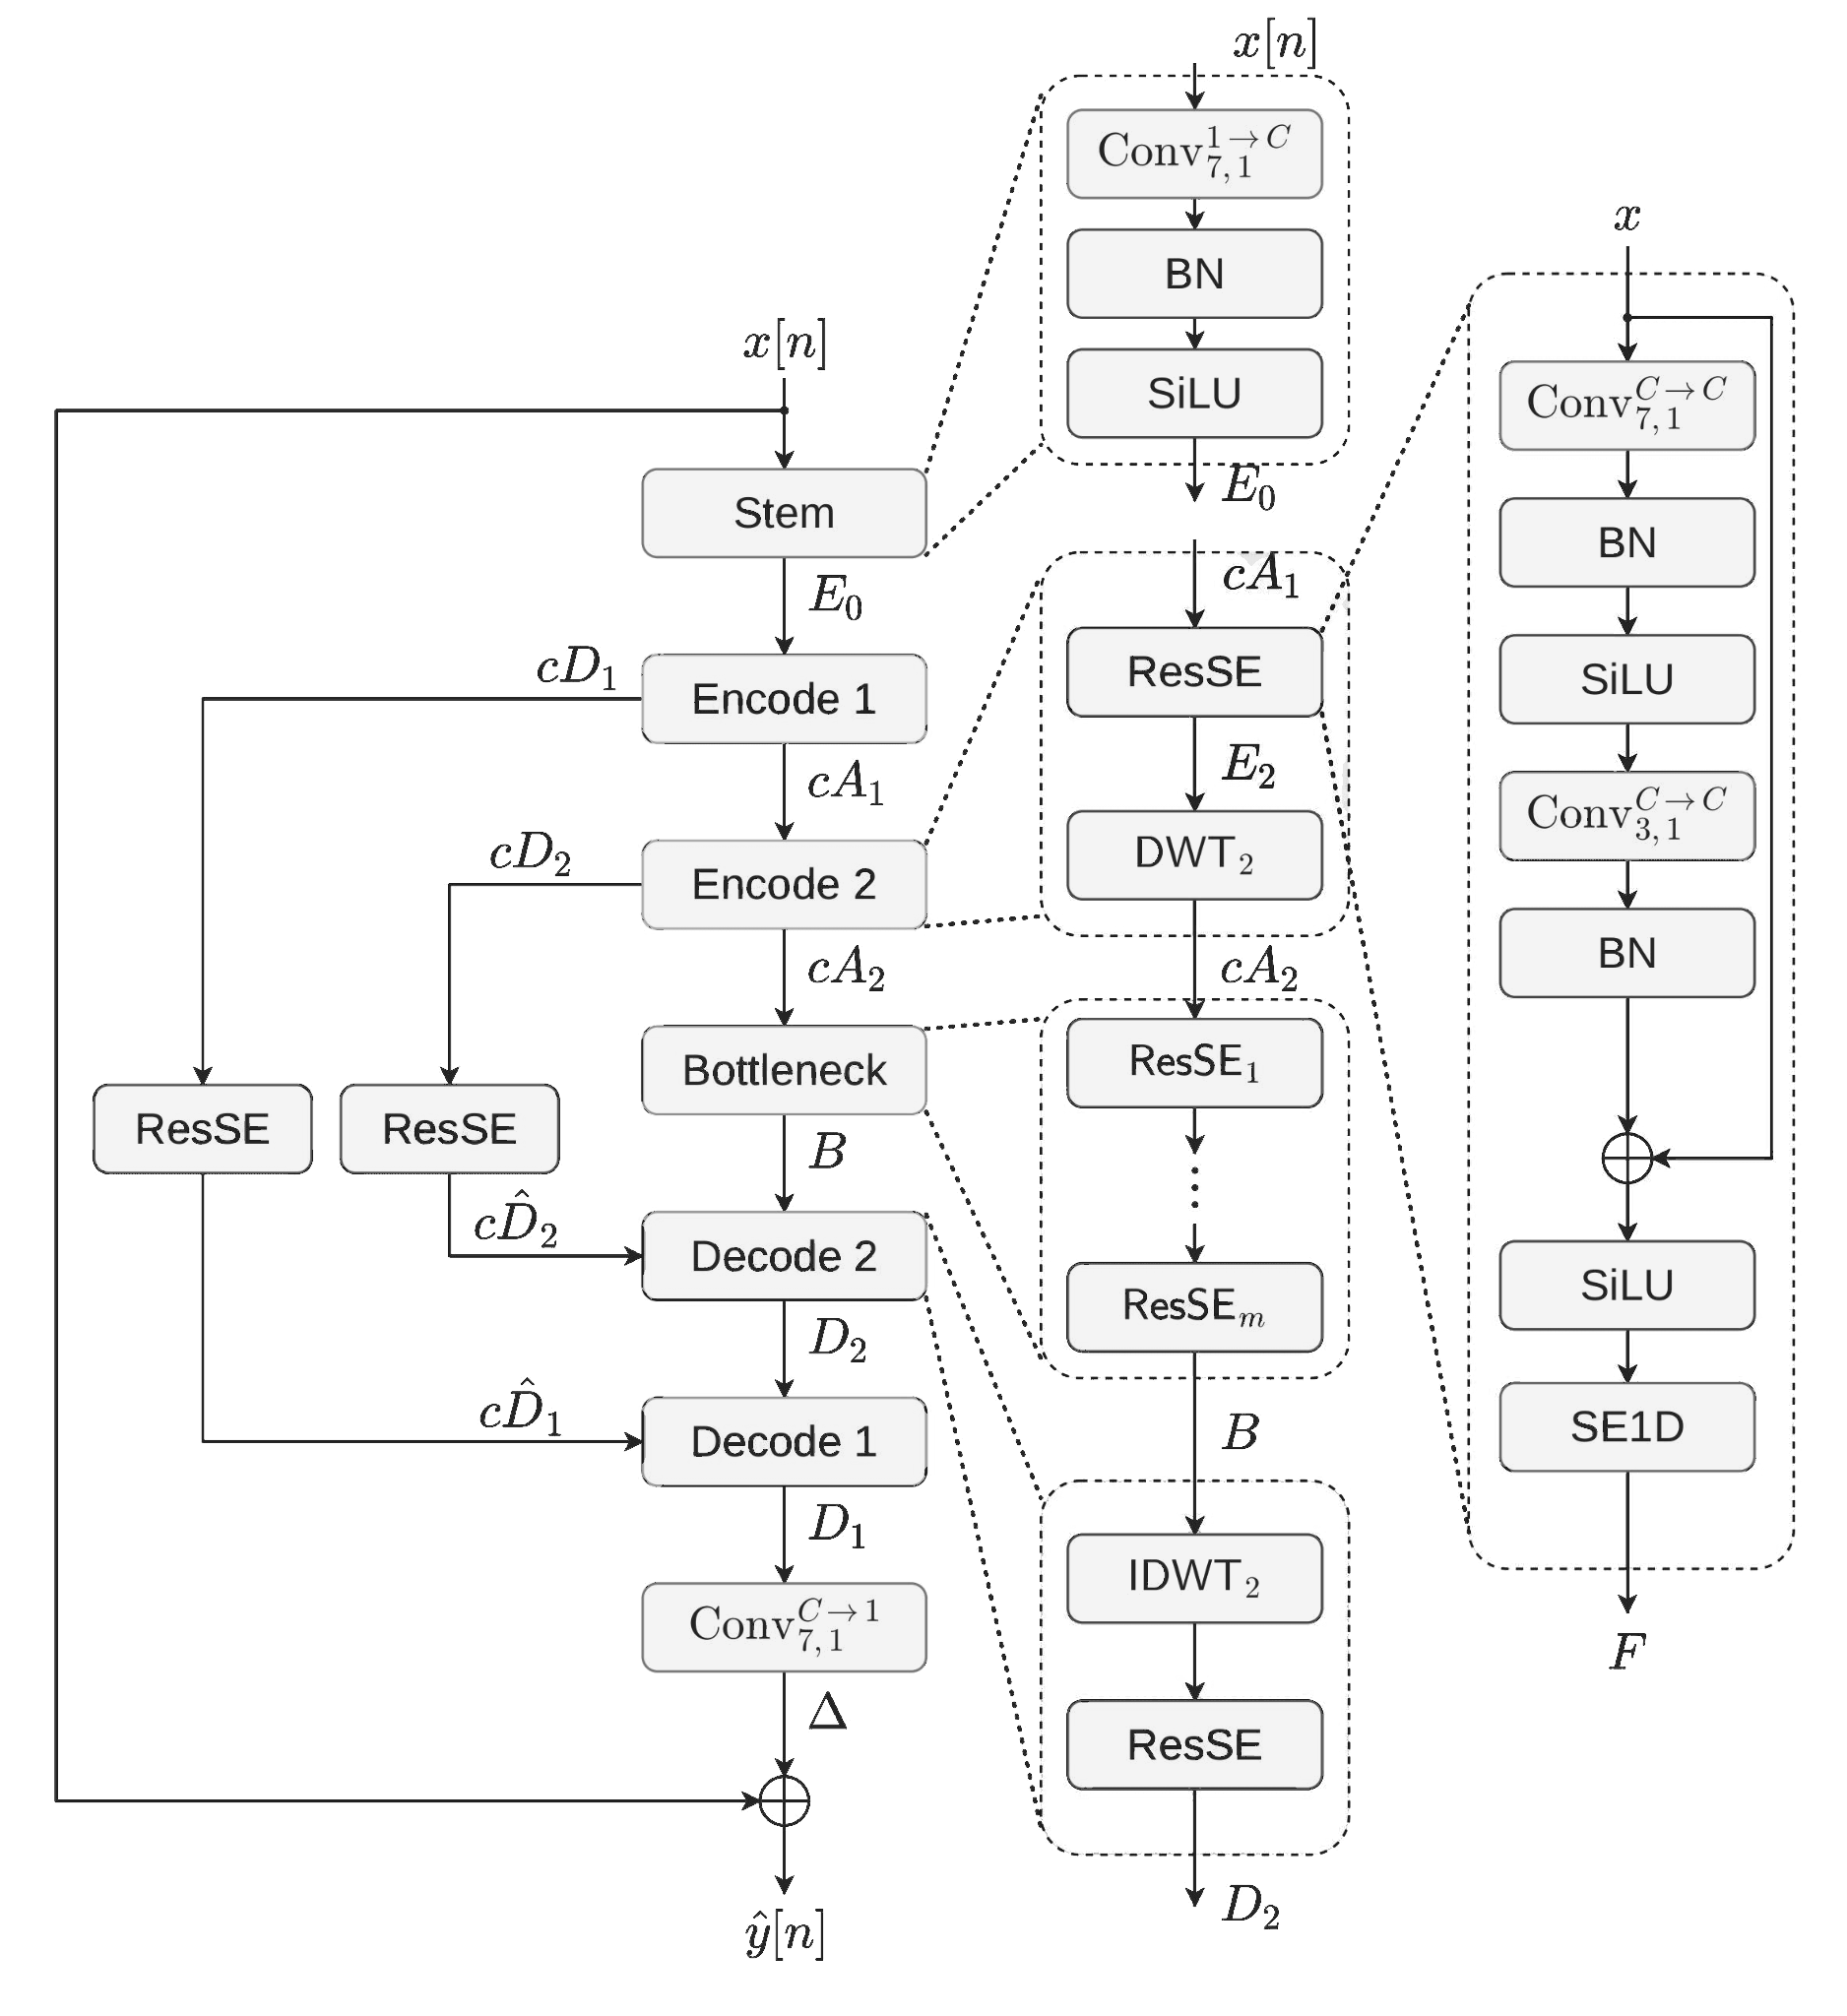
\includegraphics[width=\columnwidth]{Fig/fig2_haarsymlite.png}
\caption{Architecture of the proposed \HSL{} denoiser ($C=32$, 75{,}133 parameters). Left: the noisy segment $x[n]$ passes through the Stem, two Encode stages, the Bottleneck, two Decode stages and an output convolution, and the predicted correction $\Delta$ is added to $x[n]$ to give $\hat{y}[n]$. The detail subbands $cD_1, cD_2$ are refined by separate ResSE blocks into $c\hat{D}_1, c\hat{D}_2$ and passed to the Decode stages. Right: internal structure of the Stem, Encode 2, Bottleneck and Decode 2, and of the ResSE block with its SE1D channel attention module ($x \rightarrow F$).}
\label{fig:haarsymlite}
\end{figure}

\subsection{Stage 1: \HSL{} Architecture}
\label{sec:haarsymlite}
\HSL{} maps a noisy segment $x[n] \in \mathbb{R}^{1 \times L}$ to a denoised estimate $\hat{y}[n] \in \mathbb{R}^{1 \times L}$ through an encoder--bottleneck--decoder structure with two Haar wavelet levels (Fig.~\ref{fig:haarsymlite}). The input is first projected into a $C$-channel feature space by a convolutional stem:
\begin{equation}
\begin{gathered}
E_0 = \mathrm{SiLU}\Big(\mathrm{BN}\big(\mathrm{Conv}_{7,1}^{1 \to C}(x[n])\big)\Big), \\
E_0 \in \mathbb{R}^{C \times L},
\end{gathered}
\end{equation}
where $\mathrm{Conv}_{k,s}^{C_{\mathrm{in}} \to C_{\mathrm{out}}}$ denotes a 1D convolution with kernel size $k$ and stride $s$, $\mathrm{BN}(\cdot)$ denotes batch normalization and $\mathrm{SiLU}(\cdot)$ denotes the sigmoid linear unit. All convolutions use stride one with padding that preserves the temporal length, and $C = 32$.

The main computational unit of \HSL{} is a residual block with squeeze-and-excitation, denoted as $\mathrm{ResSE}(\cdot)$. For an input $x \in \mathbb{R}^{C \times T}$, two convolutions with kernel sizes $7$ and $3$ are combined with an identity shortcut:
\begin{align}
U_1 &= \mathrm{SiLU}\Big(\mathrm{BN}\big(\mathrm{Conv}_{7,1}^{C \to C}(x)\big)\Big), \\
U_2 &= \mathrm{BN}\big(\mathrm{Conv}_{3,1}^{C \to C}(U_1)\big), \\
U_3 &= \mathrm{SiLU}(x + U_2).
\end{align}
The SE1D module then recalibrates the channel responses of $U_3$. The squeeze operation summarizes the $c$-th channel by global average pooling,
\begin{equation}
z_c = \frac{1}{T}\sum_{t=1}^{T} U_3(c,t), \quad c = 1, 2, \dots, C,
\end{equation}
and the excitation operation learns channel weights through two pointwise convolutions:
\begin{equation}
a = \sigma\Big(\mathrm{Conv}_{1,1}^{C_r \to C}\big(\mathrm{SiLU}(\mathrm{Conv}_{1,1}^{C \to C_r}(z))\big)\Big),
\end{equation}
where $z = [z_1, z_2, \dots, z_C] \in \mathbb{R}^{C \times 1}$, $C_r = \max(4, \lfloor C/r \rfloor)$ with $r = 8$, and $\sigma(\cdot)$ is the sigmoid function. The block output is obtained by channel-wise multiplication:
\begin{equation}
\begin{gathered}
F_c = a_c\, U_3(c,\cdot), \\
F = [F_1, F_2, \dots, F_C] \in \mathbb{R}^{C \times T}.
\end{gathered}
\end{equation}
Thus, $\mathrm{ResSE}(x) = F$ preserves both the channel dimension and the temporal length.

Each encoder stage consists of one $\mathrm{ResSE}$ block followed by a one-level Haar DWT. In the first encoder stage,
\begin{equation}
E_1 = \mathrm{ResSE}(E_0), \quad E_1 \in \mathbb{R}^{C \times L},
\end{equation}
and the DWT splits $E_1$ into a low-frequency approximation and a high-frequency detail:
\begin{equation}
\begin{gathered}
cA_1 = \DWT_{\mathrm{low}}(E_1), \quad cD_1 = \DWT_{\mathrm{high}}(E_1), \\
cA_1, cD_1 \in \mathbb{R}^{C \times L/2}.
\end{gathered}
\end{equation}
For a channel $h$ of the input feature, the Haar operators are $\DWT_{\mathrm{low}}(h)[n] = \frac{1}{\sqrt{2}}(h[2n] + h[2n+1])$ and $\DWT_{\mathrm{high}}(h)[n] = \frac{1}{\sqrt{2}}(h[2n+1] - h[2n])$, applied independently to every channel. Since the Haar filters are fixed, the DWT halves the temporal length without trainable parameters. The second encoder stage operates on the low-frequency branch $cA_1$:
\begin{equation}
E_2 = \mathrm{ResSE}(cA_1), \quad E_2 \in \mathbb{R}^{C \times L/2},
\end{equation}
\begin{equation}
\begin{gathered}
cA_2 = \DWT_{\mathrm{low}}(E_2), \quad cD_2 = \DWT_{\mathrm{high}}(E_2), \\
cA_2, cD_2 \in \mathbb{R}^{C \times L/4}.
\end{gathered}
\end{equation}

The detail subbands bypass the bottleneck and are refined by dedicated skip blocks:
\begin{equation}
c\hat{D}_1 = \mathrm{ResSE}(cD_1), \quad c\hat{D}_2 = \mathrm{ResSE}(cD_2).
\end{equation}
The bottleneck refines the deepest approximation $cA_2$ with a stack of $m$ residual blocks:
\begin{equation}
\begin{gathered}
B = \mathrm{ResSE}_m\big(\cdots \mathrm{ResSE}_1(cA_2)\big), \\
B \in \mathbb{R}^{C \times L/4}.
\end{gathered}
\end{equation}

The decoder mirrors the encoder: each stage applies an IDWT followed by one $\mathrm{ResSE}$ block. Although Fig.~\ref{fig:haarsymlite} draws $c\hat{D}_k$ only up to the corresponding decoder stage, $c\hat{D}_k$ is used as the high-frequency input of $\IDWT_k$, while the output of the previous stage is used as the low-frequency input:
\begin{equation}
\begin{gathered}
D_2 = \mathrm{ResSE}\big(\IDWT_2(B, c\hat{D}_2)\big), \\
D_2 \in \mathbb{R}^{C \times L/2},
\end{gathered}
\end{equation}
\begin{equation}
\begin{gathered}
D_1 = \mathrm{ResSE}\big(\IDWT_1(D_2, c\hat{D}_1)\big), \\
D_1 \in \mathbb{R}^{C \times L}.
\end{gathered}
\end{equation}
For a low-frequency input $p$ and a high-frequency input $q$, the Haar IDWT reconstructs $\IDWT(p, q)[2n] = \frac{1}{\sqrt{2}}(p[n] - q[n])$ and $\IDWT(p, q)[2n+1] = \frac{1}{\sqrt{2}}(p[n] + q[n])$, which exactly inverts the DWT and doubles the temporal length.

Finally, the denoised signal is obtained through global residual learning:
\begin{equation}
\begin{gathered}
\Delta = \mathrm{Conv}_{7,1}^{C \to 1}(D_1), \\
\hat{y}[n] = x[n] + \Delta[n].
\end{gathered}
\end{equation}
Overall, the low-frequency path carries the coarse cardiac morphology through the bottleneck, while the filtered detail subbands restore sharp QRS components during inverse wavelet reconstruction. The network predicts only the correction $\Delta$ to the noisy input.

The network is optimized end-to-end via a composite time-domain mixed loss:
\begin{equation}
\mathcal{L}_{\mathrm{mixed}}(\hat{y}, x_0) = \alpha \mathcal{L}_{\mathrm{MSE}}(\hat{y}, x_0) + (1-\alpha) \mathcal{L}_{L_1}(\hat{y}, x_0),
\label{eq:mixed_loss}
\end{equation}
where $\alpha = 0.8$. The $\mathcal{L}_{\mathrm{MSE}}$ term enforces high global signal-to-noise ratio, while the $\mathcal{L}_{L_1}$ term penalizes absolute errors linearly, mitigating the R-peak blunting caused by quadratic MSE penalties on large amplitudes.

\begin{figure}[!t]
\centering
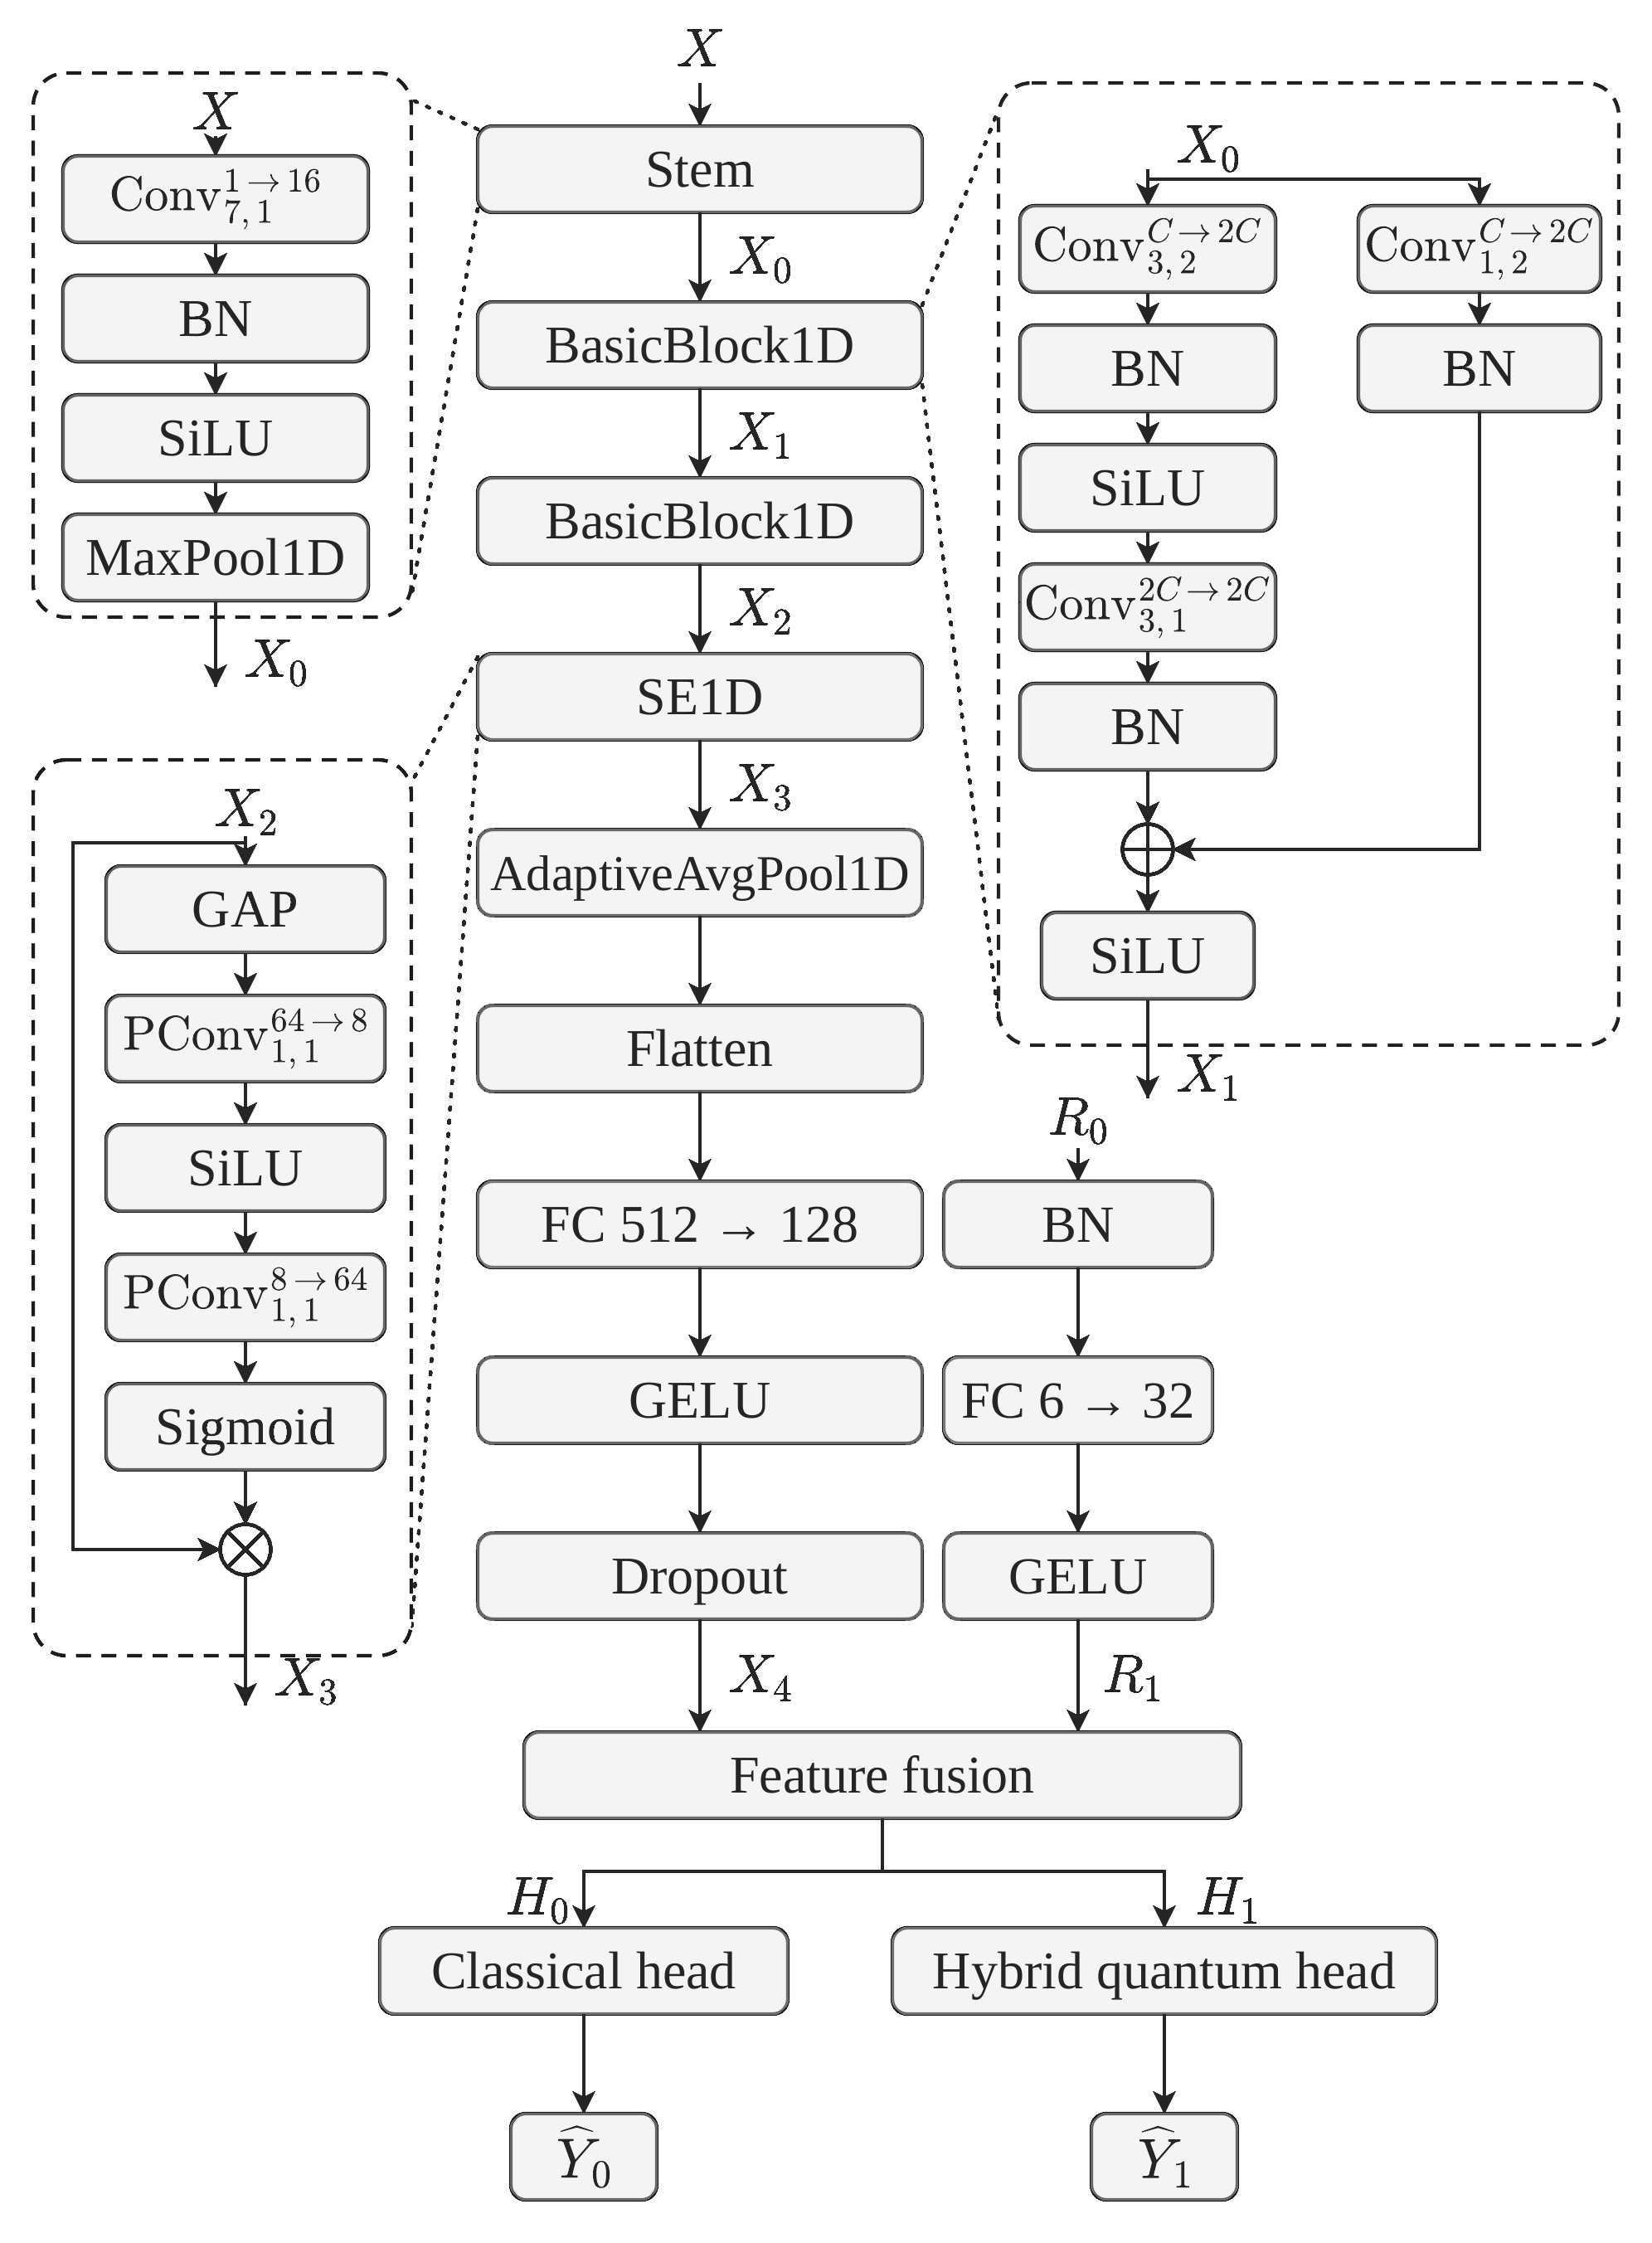
\includegraphics[width=\columnwidth]{Fig/fig3_classifier_vqc.png}
\caption{Downstream arrhythmia classification architecture (\RRN). Morphology and RR fusion network: 256-sample denoised beats pass through a 1D ResNet encoder with SE1D attention ($128\text{D}$), concatenated with an independent 6D RR-interval rhythm pathway ($32\text{D}$) to form a $160\text{D}$ feature vector.}
\label{fig:classifier}
\end{figure}

\subsection{Stage 2: Beat Classification with \RRN}
\label{sec:classifier}
\subsubsection{Beat Segmentation and Normalization}
Following R-peak locations from reference annotations, individual beats are segmented into windows of $N_b = 256$ samples centered at the R-peak (approximately $0.71$\,s), encompassing the full P-QRS-T complex. The frozen, fully convolutional denoiser is applied directly to each beat in physical millivolts, and the denoised beat $x_d$ is then standardized by a per-beat Z-score normalization: $\tilde{x} = (x_d - \mu) / (\sigma + \epsilon)$, where $\mu$ and $\sigma$ are the mean and standard deviation of the beat and $\epsilon = 10^{-6}$.

\textbf{Morphology encoder.} The normalized beat $X=\tilde{x}\in\mathbb{R}^{1\times 256}$ is encoded by a 1D ResNet with SE1D attention (Fig.~\ref{fig:classifier}). A stem ($\mathrm{Conv}_{7,1}^{1\to 16}$, BN, SiLU, max-pooling) produces $X_0$. Two BasicBlock1D residual blocks follow, each doubling the channels through a stride-2 convolution path and a projected shortcut, giving $X_1$ and $X_2$ with 64 channels. The SE1D module recalibrates the channels of $X_2$ through a $64\to 8\to 64$ pointwise-convolution bottleneck with sigmoid gating, giving $X_3$. Adaptive average pooling and flattening yield a 512D vector, which a fully connected layer ($512\to 128$) with GELU and dropout maps to the morphology embedding $X_4\in\mathbb{R}^{128}$.

\subsubsection{Independent RR-Interval Pathway}
Because supraventricular ectopic beats (S-class) are morphologically identical to normal beats in single-lead recordings, timing context is decisive. We extract six RR intervals:
\begin{equation}
f_1 = \frac{\mathrm{pre\_RR}}{f_s}, \quad f_2 = \frac{\mathrm{post\_RR}}{f_s}, \quad f_3 = \frac{\mathrm{pre\_RR}}{\overline{RR}_{\mathrm{loc}}},
\end{equation}
\begin{equation}
f_4 = \frac{\mathrm{post\_RR}}{\overline{RR}_{\mathrm{loc}}}, \quad f_5 = \frac{\mathrm{pre\_RR}}{\overline{RR}_{\mathrm{glob}}}, \quad f_6 = \frac{\mathrm{post\_RR}}{\overline{RR}_{\mathrm{glob}}},
\end{equation}
where $\overline{RR}_{\mathrm{loc}}$ is the local moving average of the RR intervals over the preceding beats, and $\overline{RR}_{\mathrm{glob}}$ is the global record average. The six features form the rhythm input $R_0=[f_1,\dots,f_6]$, which passes through a dedicated pathway ($\mathrm{BatchNorm1D} \to \mathrm{Linear}(6 \to 32) \to \mathrm{GELU}$) to give $R_1\in\mathbb{R}^{32}$. Feature fusion concatenates it with the 128D morphology embedding $X_4$, forming a $160\text{D}$ joint embedding $h=[X_4;R_1] \in \mathbb{R}^{160}$, which is fed unchanged to both heads ($H_0=H_1=h$ in Fig.~\ref{fig:classifier}).

\subsubsection{Dual Interchangeable Classification Heads}
\RRN{} supports two interchangeable heads, producing the class logits $\hat{Y}_0$ (classical) and $\hat{Y}_1$ (hybrid quantum) in Fig.~\ref{fig:classifier}:
\begin{enumerate}
    \item \textbf{Classical MLP Head:} A 3-layer fully connected network ($160 \to 128 \to 128 \to 3$) with GELU activations ($37{,}507$ parameters).
    \item \textbf{Hybrid Quantum Head (VQC):} The 160D vector is compressed to 64D and mapped into the Hilbert state space of 6 qubits ($2^6 = 64$) via amplitude encoding:
    \begin{equation}
    |\psi_{\mathrm{in}}\rangle = \sum_{i=0}^{63} x_i |i\rangle, \quad \sum_{i=0}^{63} |x_i|^2 = 1.
    \end{equation}
    A 2-layer parameterized quantum circuit applies single-qubit rotations $R_y(\theta), R_z(\phi)$ followed by a closed cyclic ring of CNOT entangling gates ($q_i \to q_{(i+1)\bmod 6}$), requiring only $2 \times 6 \times 2 = 24$ trainable quantum parameters. Twelve expectation values (6 single Pauli-Z $\langle Z_i \rangle$ and 6 nearest-neighbor correlations $\langle Z_i Z_{i+1} \rangle$) are measured and combined with a parallel 64D classical residual bypass:
    \begin{equation}
    \ell_{\mathrm{qnt}} = W_2 \cdot \mathrm{GELU}\Big(W_1 \big[\langle Z \rangle_{12}; \mathrm{GELU}(W_b h)\big]\Big),
    \end{equation}
    which safeguards against quantum barren plateaus \cite{mcclean2018}. The total hybrid head comprises $30{,}875$ trainable parameters and is simulated using PennyLane \cite{pennylane2018}.
\end{enumerate}

\subsubsection{Imbalance Handling and Soft-Voting Ensemble}
To handle severe class imbalance between normal beats and rare arrhythmias, training samples are drawn using a weighted random sampler with sampling weights $w_c \propto n_c^{-p}$ ($p=0.9$). For each configuration, 5 independent seeds (0 to 4) are trained and aggregated via a Soft-Voting Ensemble:
\begin{equation}
\hat{p}_{\mathrm{ens}}(c \mid x) = \frac{1}{5}\sum_{s=0}^4 \mathrm{softmax}\big(\ell^{(s)}(x)\big)_c.
\end{equation}
